\section{Analyse der Performance}

Es wurden ein paar sehr grundlegende Untersuchungen bezüglich der Abhängigkeiten des Programs von $n$ und $k$ durchgeführt.

\subsection{Einwicklung der Lösungsgüte}

Für verschiedene $n$ und $k$ Paare wurde zufällig ein Problem generiert und anschließend unterschied wie lange die Algorithm benötigen um Lösungen für dieses Problem zu finden. Die Güte der Lösungen wird dabei im Verhältnis zur optimalen Lösung angegeben (Die mittels clingo gefunden werden kann).

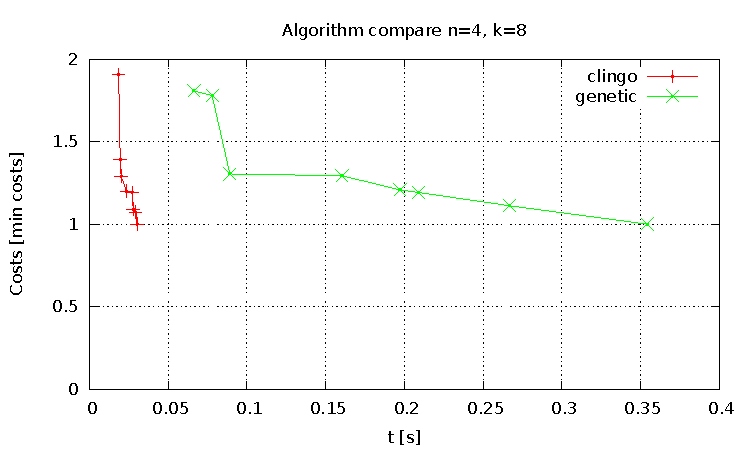
\includegraphics{../../plots/algorithmCompare-n4-k8.pdf}

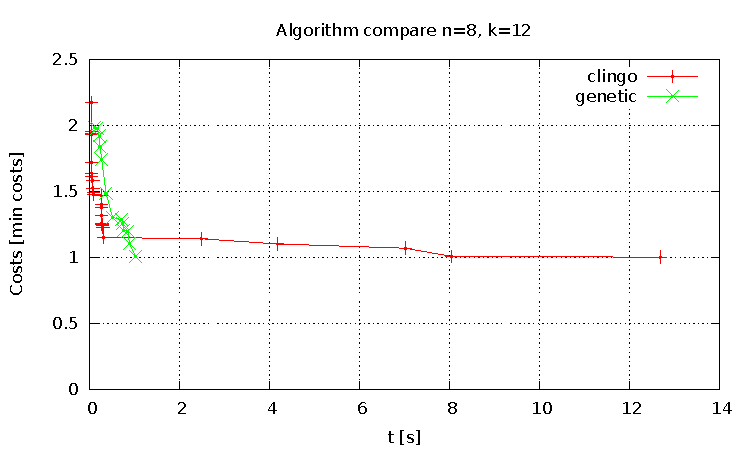
\includegraphics{../../plots/algorithmCompare-n8-k12.pdf}

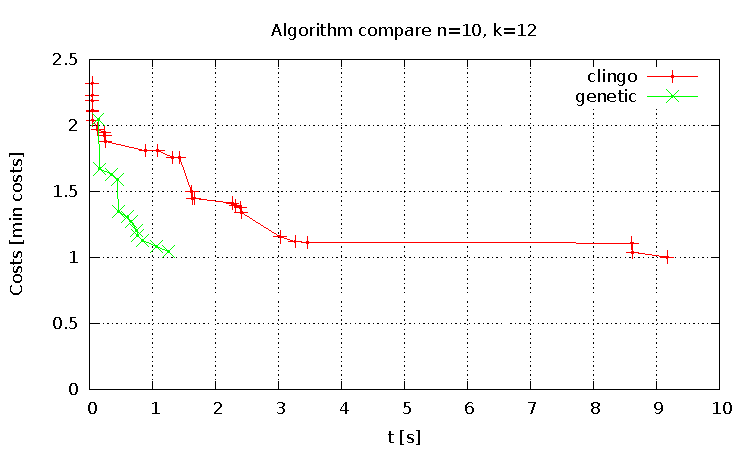
\includegraphics{../../plots/algorithmCompare-n10-k12.pdf}


Es ist gut zu erkennen, dass die Algorithm mit einer relativ schlechten Lösung anfangen und sich dann sehr schnell der optimalen Lösung annähern. Die Laufzeit von Clingo hängt sehr stark von der Umfang des Problems ab, während der genetische Algorithmus deutlich konstanter in der Laufzeit ist.


\subsection{Abhängigkeit von k}

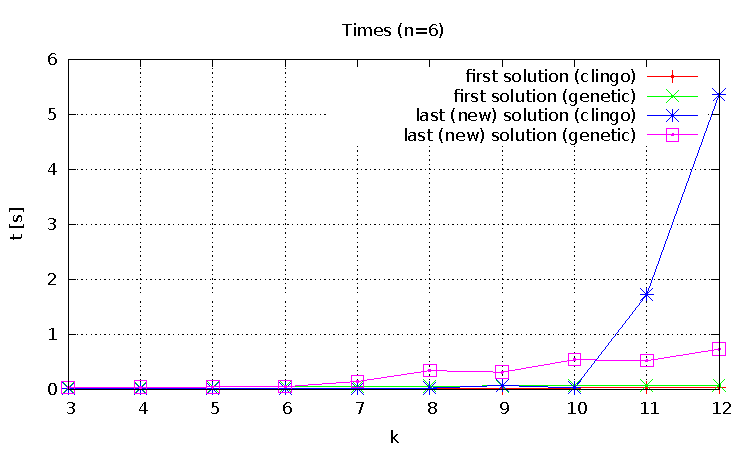
\includegraphics{../../plots/timesPerK-n6.pdf}

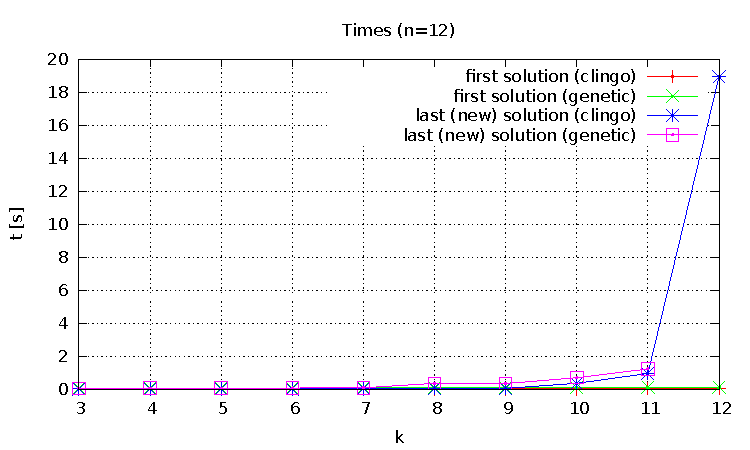
\includegraphics{../../plots/timesPerK-n12.pdf}


\subsection{Abhängigkeit von n}


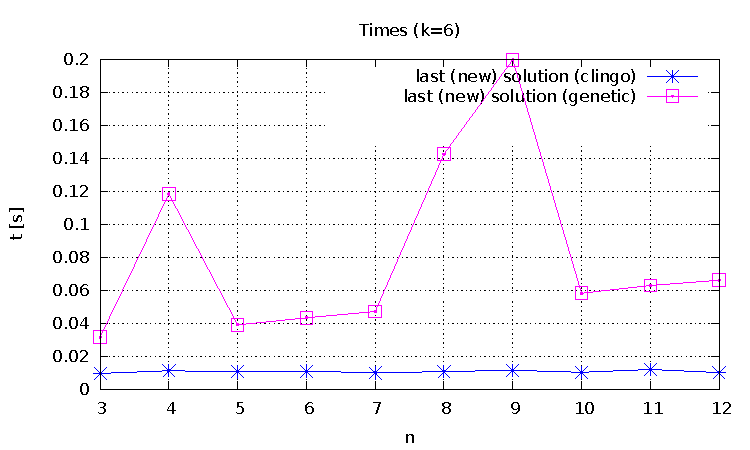
\includegraphics{../../plots/timesPerN-k6.pdf}

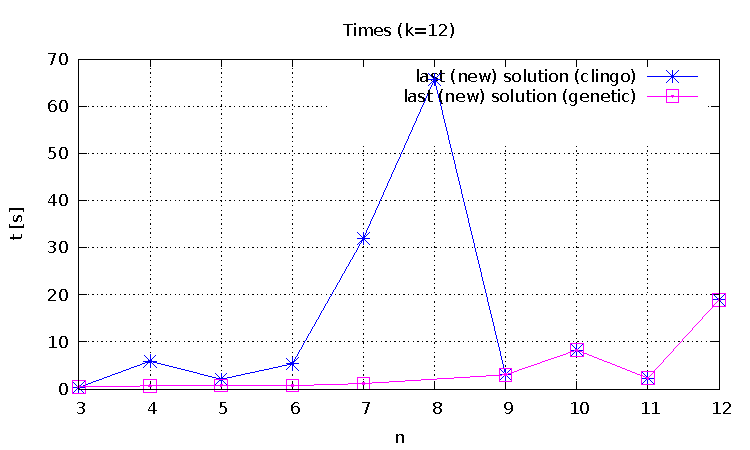
\includegraphics{../../plots/timesPerN-k12.pdf}

